The following algorithm finds all possible partitions $\mathfrak{S}$ on $\mathcal{C}$ based on forming STAs into trees on the basis of orthogonality.

It is assumed that any given STA cannot belong to more than one SUS group. A scheduling scheme that allocates temporal resources to the groups developed here is not discussed. The algorithm could be modified to allow an STA to belong to more than one SUS group. This would likely make scheduling fairness more difficult.

\textbf{Conceptual description:}
\begin{enumerate}
    \item For each STA $k \in \mathcal{C}$, find the set of STAs who are semi-orthogonal to $k$ such that $\mathcal{S}_k = \lbrace j\ : \ \vert \textbf{h}_k \textbf{h}_j^H \vert < \alpha \rbrace \ \forall j \neq k,\ k = 1,2,3\ldots\vert\mathcal{C}\vert$
    \item Build a tree for each $k$ that represents potential SUS groups that contain $k$
    \item Form SUS group sets based on the traversal of each tree
    \item Remove all SUS group sets that are larger than the number of antennas available at the AP
    \item Form $\mathfrak{S}$ by permuting the sets produced by tree traversals while making sure that STAs are not duplicated in groups.
\end{enumerate}

Each group of semi-orthogonal STAs belonging to $k$, $\mathcal{S}_k$ is formed into a tree. The trees are structured using the following algorithm.
\begin{enumerate}
    \item Place $k$ at the root of the tree
    \item Write the first STA $l \in \mathcal{S}_k$ as the child of $k$.
    \item Repeat the previous step adding children to the current branch of the tree so long as the orthogonal sets intersect with all of the parent nodes of the tree. Add a child node to the branch for every STA $j : j \in \mathcal{S}_k \cap j \in \mathcal{S}_l$. Once $j$ has been added to the tree remove $j$ from $\mathcal{S}_k$.
    For example, given three STAs $A,B,C$, then $A$'s tree will be three deep if $B\in\mathcal{S}_A \cap C\in \mathcal{S}_A \cap C \in \mathcal{S}_B$. In other words, A,B,C are mutually semi-orthogonal to each other.
\end{enumerate}

SUS groups containing $k$ are generated by permuting the nodes that exist on any branch between the root and leaf node. The permutations must include the root of the tree. Permuting the traversals of a tree generated from $\mathcal{S}_k$ will give all the possible SUS groups that contain $k$.

Finally, each of the SUS groups generated for a given STA are permuted with each other to generate $\mathfrak{S}$. Assuming that each STA must be included in $\mathfrak{S}$ once and only once, the SUS groups generated from a tree are muted once the STA at the root of that tree is included in a previous SUS group.

\begin{figure}
    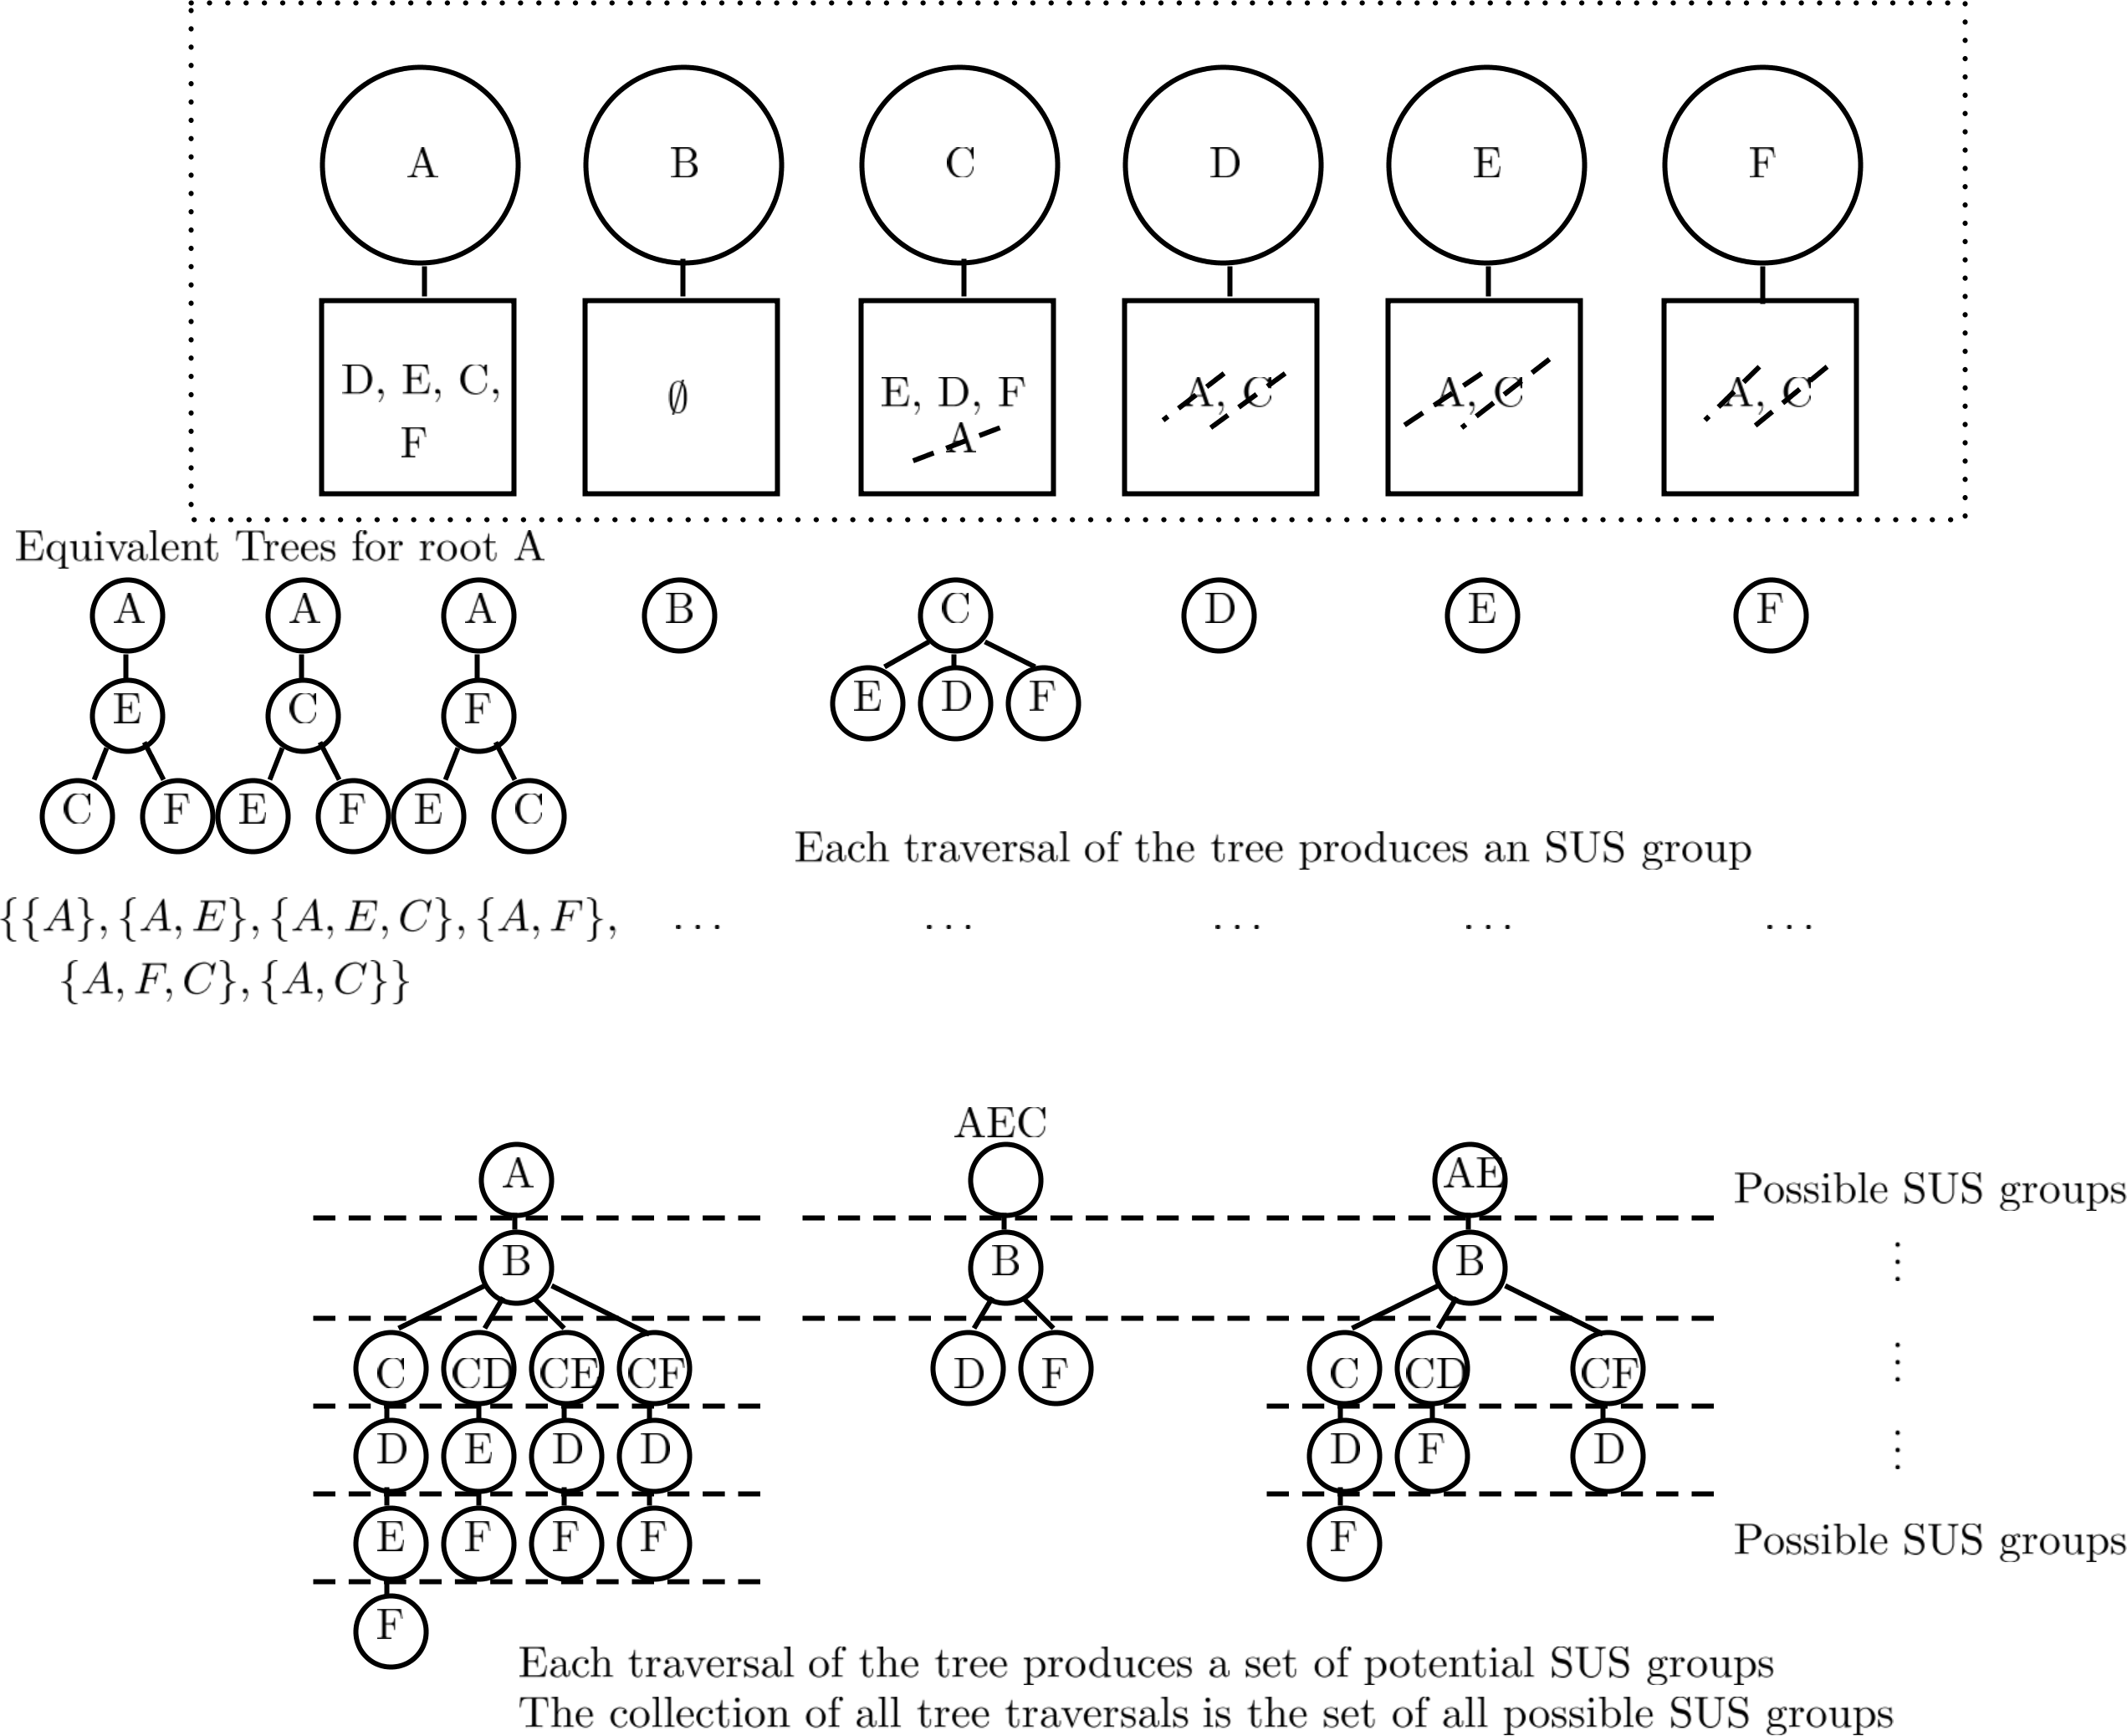
\includegraphics[width=16cm]{figs/exhastive_tree_alg.png}\\
    \caption{Diagram of the T-SUS algorithm}
    \label{fig:tree_alg}
\end{figure}